\documentclass[portrait,final]{baposter}
%\documentclass[a4shrink,portrait,final]{baposter}
% Usa a4shrink for an a4 sized paper.

\tracingstats=2

\usepackage{verbatim} 
\usepackage{times}
\usepackage{calc}
\usepackage{graphicx}
\usepackage{amsmath}
\usepackage{amssymb}
\usepackage{relsize}
\usepackage{multirow}
\usepackage{bm}
\usepackage{epsfig}
\usepackage{graphicx}
\usepackage{multicol}
\usepackage{url}
\usepackage{cite}
\usepackage{pgfbaselayers}
\usepackage{algorithm,algorithmic}
\usepackage{tikz}
\usetikzlibrary{shapes,arrows}

\usepackage{array}
\usepackage{amsmath}
\usepackage{ulem}
\usepackage{pgflibraryshapes}  
\usetikzlibrary{shapes,arrows,snakes,backgrounds}
\usepackage[overlay,absolute]{textpos}
\usepackage[latin1]{inputenc}
\usepackage[english]{babel}
\usepackage{listings}
\usepackage{pgfpages}






\pgfdeclarelayer{background}
\pgfdeclarelayer{foreground}
\pgfsetlayers{background,main,foreground}
\usetikzlibrary{shapes,arrows}
\usepackage{helvet}
\usepackage{palatino}

\newcommand{\captionfont}{\footnotesize}

\selectcolormodel{cmyk}

\graphicspath{{images/}}

%%%%%%%%%%%%%%%%%%%%%%%%%%%%%%%%%%%%%%%%%%%%%%%%%%%%%%%%%%%%%%%%%%%%%%%%%%%%%%%%
% Multicol Settings
%%%%%%%%%%%%%%%%%%%%%%%%%%%%%%%%%%%%%%%%%%%%%%%%%%%%%%%%%%%%%%%%%%%%%%%%%%%%%%%%
\setlength{\columnsep}{0.7em}
\setlength{\columnseprule}{0mm}


%%%%%%%%%%%%%%%%%%%%%%%%%%%%%%%%%%%%%%%%%%%%%%%%%%%%%%%%%%%%%%%%%%%%%%%%%%%%%%%%
% Save space in lists. Use this after the opening of the list
%%%%%%%%%%%%%%%%%%%%%%%%%%%%%%%%%%%%%%%%%%%%%%%%%%%%%%%%%%%%%%%%%%%%%%%%%%%%%%%%
\newcommand{\compresslist}{%
\setlength{\itemsep}{1pt}%
\setlength{\parskip}{0pt}%
\setlength{\parsep}{0pt}%
}

\newcommand{\opal}{\textsc{OPAL}}
\newcommand{\opalt}{\textsc{OPAL-t }}
\newcommand{\opalcycl}{\textsc{OPAL-cycl}}
\newcommand{\opalmap}{\textsc{OPAL-map }}
\newcommand{\opalenv}{\textsc{OPAL-envelop}}

\newcommand{\mad}{\textsc{mad }}
\newcommand{\madnine}{\textsc{mad9 }}
\newcommand{\madninep}{\textsc{mad9p }}
\newcommand{\madeight}{\textsc{mad8 }}

\newcommand{\classic}{\textsc{classic }}
\newcommand{\hfifepart}{\textsc{H5Part }}
\newcommand{\hfifefe}{\textsc{H5FED }}

\renewcommand{\epsilon}{\varepsilon} 
\renewcommand{\vec}[1]{{\bf #1}} 
\newcommand{\dt}[1]{\frac{\partial #1}{\partial t}}
\newcommand{\dtt}[1]{\frac{\partial^2 #1}{\partial t^2}}
\newcommand{\dtvec}[1]{\frac{\partial {\mathbf #1}}{\partial t}}
\newcommand{\dttvec}[1]{\frac{\partial^2 {\mathbf #1}}{\partial t^2}}
\newcommand{\rot}{\vec{\nabla} \wedge }
\renewcommand{\div}{\vec{\nabla} \cdot }

\def\vec#1{\mathbf{#1}}
\def\vecg#1{\boldsymbol{#1}}
\def\norm#1{\| #1 \|} 
\def\tr{^{\!\top}}

\def\curl{{\bf curl}\,}
\def\curlp{{\rm curl}_p\,}
\def\div{{\rm div}\,}
\def\grad{\nabla}
\def\gradp{\nabla_p}
\def\dotp#1#2{\langle#1,#2\rangle}
\def\eps{\varepsilon}

\newcommand{\mat}[1]{\ensuremath{\boldsymbol{#1}}}
\newcommand{\vect}[1]{\ensuremath{\mathbf{#1}}}
\newcommand{\iprod}[2]{\ensuremath{\langle#1,#2\rangle}}
\newcommand{\abs}[1]{\ensuremath{|#1|}}

\newcommand{\Nedelec}{N\'{e}d\'{e}lec}

\newcommand{\id}[1]{\structure{#1}}

\newcommand {\Co}{{\mathbb{C}}}
\newcommand {\Int}{{\mathbb{Z}}}
\newcommand {\Nat}{{\mathbb{N}}}
%
%
\newcommand {\Hcurl}{{H(\mathbf{curl};\Omega)}}
\newcommand {\Hocurl}{{H_0(\mathbf{curl};\Omega)}}
\newcommand {\Hdiv}{{H(\mathrm{div};\Omega)}}
\newcommand {\Hodiv}{{H_0(\mathbf{div};\Omega)}}
%
\renewcommand {\Re}{{\rm I \kern-2pt R}}
\newcommand{\vc}[1]{\mbox{\boldmath $#1$}}
\newcommand {\RM}[1]{\mathrm{#1}}



\TPGrid[4mm,25mm]{10}{5}

\tikzstyle{format} = [draw, thin, fill=blue!20]
\tikzstyle{pblock} = [rectangle, draw, fill=blue!20, text width=6em, text centered, rounded corners, minimum height=0.4em]
\tikzstyle{mblock} = [rectangle, draw, fill=green!20, text width=6em, text centered, rounded corners, minimum height=0.4em]
\tikzstyle{bblock} = [rectangle, draw, fill=gray!20, text width=6em, text centered, rounded corners, minimum height=0.4em]
\tikzstyle{prblock} = [rectangle, draw, fill=red!20, text width=6em, text centered, rounded corners, minimum height=0.4em]
\tikzstyle{rblock} = [rectangle, draw, fill=black!50, text width=6em, text centered, rounded corners, minimum height=0.4em]
\tikzstyle{block} = [rectangle, draw, fill=gray!20, text centered, rounded corners]
\tikzstyle{decision} = [diamond, draw, fill=blue!20, text width=4.5em, text badly centered, node distance=3cm, inner sep=0pt]
\tikzstyle{medium} = [ellipse, draw, thin, fill=green!20, minimum height=2.5em]
\tikzstyle{cloud} = [draw, ellipse,fill=red!20, node distance=3cm, minimum height=2em]
\tikzstyle{line} = [draw, -latex']
\tikzstyle{emptyblock} = [rectangle]
\tikzstyle{progblock} = [rectangle, draw, fill=yellow!20, text width=6em, text centered, minimum height=0.4em]
\tikzstyle{null} = [rectangle, fill=blue!0, text width=6em, text centered, rounded corners, minimum height=0.4em]

% Figure 1
\tikzstyle{f1pblock} = [rectangle, draw, fill=blue!20, text width=5em, text centered, rounded corners, minimum height=0.4em]
\tikzstyle{f1pblockr} = [rectangle, draw, fill=red!20, text width=5em, text centered, rounded corners, minimum height=0.4em]
\tikzstyle{f1pblockw} = [rectangle, draw, text width=5em, text centered, rounded corners, minimum height=0.4em]
\tikzstyle{f1rblock} = [rectangle, draw, fill=gray!50, text width=10em, text centered, rounded corners, minimum height=0.4em]
\tikzstyle{f1medium} = [ellipse, draw, fill=green!20, text width=5em, text centered, rounded corners, minimum height=0.4em]
\tikzstyle{f1mediumr} = [ellipse, draw, thin, fill=red!20, minimum height=2.5em]
\tikzstyle{f1line} = [draw, -latex']
\tikzstyle{f1null} = [rectangle, fill=blue!0, text width=6em, text centered, rounded corners, minimum height=0.4em]






%%%%%%%%%%%%%%%%%%%%%%%%%%%%%%%%%%%%%%%%%%%%%%%%%%%%%%%%%%%%%%%%%%%%%%%%%%%%%%
%%% Begin of Document
%%%%%%%%%%%%%%%%%%%%%%%%%%%%%%%%%%%%%%%%%%%%%%%%%%%%%%%%%%%%%%%%%%%%%%%%%%%%%%

\begin{document}

%%%%%%%%%%%%%%%%%%%%%%%%%%%%%%%%%%%%%%%%%%%%%%%%%%%%%%%%%%%%%%%%%%%%%%%%%%%%%%
%%% Here starts the poster
%%%---------------------------------------------------------------------------
%%% Format it to your taste with the options
%%%%%%%%%%%%%%%%%%%%%%%%%%%%%%%%%%%%%%%%%%%%%%%%%%%%%%%%%%%%%%%%%%%%%%%%%%%%%%
% Define some colors
\definecolor{silver}{cmyk}{0,0,0,0.3}
\definecolor{yellow}{cmyk}{0,0,0.9,0.0}
\definecolor{reddishyellow}{cmyk}{0,0.22,1.0,0.0}
\definecolor{black}{cmyk}{0,0,0.0,1.0}
\definecolor{darkYellow}{cmyk}{0,0,1.0,0.5}
\definecolor{darkSilver}{cmyk}{0,0,0,0.1}

%\definecolor{lightyellow}{cmyk}{0,0,0.3,0.0}
\definecolor{lightyellow}{cmyk}{0,0,0.0,0.0}
\definecolor{lighteryellow}{cmyk}{0,0,0.0,0.0}
%\definecolor{lighteryellow}{cmyk}{0,0,0.1,0.0}
\definecolor{lighteryellow}{cmyk}{0,0,0.0,0.0}
\definecolor{lightestyellow}{cmyk}{0,0,0.0,0.0}

%%
\typeout{Poster Starts}
%\background{
%  \begin{tikzpicture}[remember picture,overlay]%
%    \draw (current page.north west)+(-2em,2em) node[anchor=north west] {\includegraphics[height=1.1\textheight]{silhouettes_background}};
%  \end{tikzpicture}%
%}

\newlength{\leftimgwidth}
\begin{poster}%
  % Poster Options
  {
  % Show grid to help with alignment
  grid=no,
  % Column spacing
  colspacing=1em,
 % columns=2,
  % Color style
  bgColorOne=lighteryellow,
  bgColorTwo=lightestyellow,
  borderColor=reddishyellow,
  headerColorOne=yellow,
  headerColorTwo=reddishyellow,
  headerFontColor=black,
  boxColorOne=lightyellow,
  boxColorTwo=black,
  % Format of textbox
  textborder=roundedleft,
  % Format of text header
  eyecatcher=yes,
  headerborder=open,
  headerheight=0.1\textheight,
  headershape=roundedright,
  headershade=plain,
  headerfont=\large\textsf, %Sans Serif
  boxshade=plain,
%  background=shade-tb,
  background=plain,
  linewidth=2pt
  }
  % Eye Catcher
  {
\includegraphics[height=5em]{logopsi}} % No eye catcher for this poster. (eyecatcher=no above). If an eye catcher is present, the title is centered between eye-catcher and logo.
  % Title
  {\sf %Sans Serif
  %\bf% Serif
   The OPAL (Object Oriented Parallel Accelerator Library) Framework 
}
  % Authors
  {\sf %Sans Serif
  % Serif
  \vspace{1em}Andreas Adelmann, Christof Kraus, Yves Ineichen (PSI), \\ Steve Russell (LANL), Yuanjie Bi and Jianjun Yang (CIAE)\\
 
 
  }
   % University logo
  {% The makebox allows the title to flow into the logo, this is a hack because of the L shaped logo.
    \makebox[8em][r]{%
      \begin{minipage}{12em}
        \hfill
        %
\includegraphics[height=4em]{psilogo}
        %\includegraphics[height=7.0em]{logo}
      \end{minipage}
    }
  }

  \tikzstyle{light shaded}=[top color=baposterBGtwo!30!white,bottom color=baposterBGone!30!white,shading=axis,shading angle=30]

  % Width of left inset image
     \setlength{\leftimgwidth}{0.78em+8.0em}

%%%%%%%%%%%%%%%%%%%%%%%%%%%%%%%%%%%%%%%%%%%%%%%%%%%%%%%%%%%%%%%%%%%%%%%%%%%%%%
%%% Now define the boxes that make up the poster
%%%---------------------------------------------------------------------------
%%% Each box has a name and can be placed absolutely or relatively.
%%% The only inconvenience is that you can only specify a relative position 
%%% towards an already declared box. So if you have a box attached to the 
%%% bottom, one to the top and a third one which should be in between, you 
%%% have to specify the top and bottom boxes before you specify the middle 
%%% box.
%%%%%%%%%%%%%%%%%%%%%%%%%%%%%%%%%%%%%%%%%%%%%%%%%%%%%%%%%%%%%%%%%%%%%%%%%%%%%%
    %
    % A coloured circle useful as a bullet with an adjustably strong filling
    \newcommand{\colouredcircle}[1]{%
      \tikz{\useasboundingbox (-0.2em,-0.32em) rectangle(0.2em,0.32em); \draw[draw=black,fill=baposterBGone!80!black!#1!white,line width=0.03em] (0,0) circle(0.18em);}}

%%%%%%%%%%%%%%%%%%%%%%%%%%%%%%%%%%%%%%%%%%%%%%%%%%%%%%%%%%%%%%%%%%%%%%%%%%%%%%
  \headerbox{Motivation and Introduction}{name=abstract,column=0,row=0,span=3}{
%%%%%%%%%%%%%%%%%%%%%%%%%%%%%%%%%%%%%%%%%%%%%%%%%%%%%%%%%%%%%%%%%%%%%%%%%%%%%%
\sf  \opal is a tool for charged-particle optics in
accelerator structures and beam lines. 
Using the \mad\ language with extensions, \opal is derived from \madninep\ and is based 
on the CLASSIC class library. IPPL (Independent Parallel Particle Layer) is
the framework which provides parallel particles and fields using data parallel ansatz. Other libraries such as GSL and Trilinos covering efficiently various aspects of numerical computations.

\opal is built from the ground up as a parallel application exemplifying the fact that HPC (High Performance Computing) 
is the third leg of science, complementing theory and the experiment. 
HPC is made possible now through the increasingly sophisticated mathematical models and evolving computer power available on the desktop
and in super computer centers. \opal runs on your laptop as well as on the largest HPC clusters available today.

OPAL comes in the following flavors:
\begin{itemize}
\item \opalcycl tracks particles with 3D space charge including neighboring turns and particle matter models
\item \opalt can be used to model guns, injectors and complete FEL's excluding the undulator
\item  \opalenv particle bunches represented by elliptical slices, a low dimensional, but very fast model for the design and operation of FEL's.
\end{itemize}
Documentation and quality assurance are given our highest attention since we are convinced that adequate documentation 
is a key factor in the usefulness of a code like \opal to study present and future particle accelerators. 
Using tools such as a source code version control system, source code documentation, nightly regression tests and an extensive user manual, we are committed to providing users as well as co-developers with state-of-the-art documentation to \opal.
\vspace{0.3em}
 }

%%%%%%%%%%%%%%%%%%%%%%%%%%%%%%%%%%%%%%%%%%%%%%%%%%%%%%%%%%%%%%%%%%%%%%%%%%%%%%
  \headerbox{Architecture of \opal}{name=model,column=0,span=2,below=abstract}{
%%%%%%%%%%%%%%%%%%%%%%%%%%%%%%%%%%%%%%%%%%%%%%%%%%%%%%%%%%%%%%%%%%%%%%%%%%%%%%
\begin{center}
 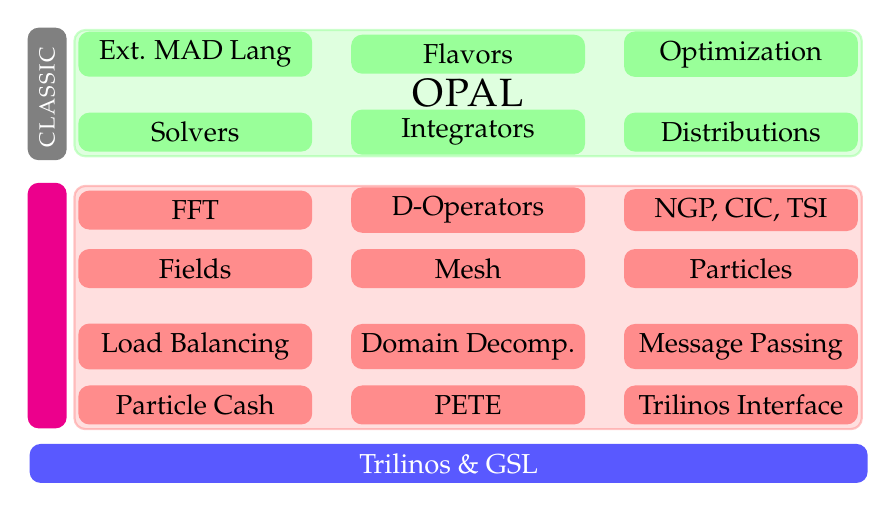
\begin{tikzpicture}[scale=0.99, transform shape]
    
      \begin{scope}[shape=rectangle,rounded corners,minimum width=3.0cm,minimum height=0.5cm,fill=yellow,text centered]
      
      \draw[rounded corners, draw=green!40, thick, fill=green!25, opacity=0.5, text centered] (-1.55, 1.31) rectangle (8.55,-0.31) node[black, thick, anchor=center, opacity=1., font=\Large] at (3.5, 0.5) {\opal};
      \node[fill= green!40] (0_00) at (0.0,1.0) {Ext. MAD Lang};
      \node[fill= green!40] (0_00) at (3.5,1.0) {Flavors};
      \node[fill= green!40] (0_00) at (7.0,1.0) {Optimization};
      \node[fill= green!40] (0_00) at (0,0.0)   {Solvers};
      \node[fill= green!40] (0_00) at (3.5,0.0) {Integrators};
      \node[fill= green!40] (0_00) at (7.0,0.0) {Distributions};

 \draw[rounded corners, draw=red!45, thick, fill=red!25, opacity=0.5, text centered] (-1.55, -0.69) rectangle (8.55,-3.81) 
                 node[black, thick, anchor=center, opacity=1.0, font=\Large] at (3.5, -2.25) {\ippl};
       \node[fill= red!45] (q_00) at (0,-1) {FFT};
       \node[fill= red!45] (q_01) at (3.5,-1) {D-Operators};
       \node[fill= red!45] (q_02) at (7,-1) {NGP, CIC, TSI};
       \node[fill= red!45] (q_10) at (0,-1.75) {Fields};
       \node[fill= red!45] (q_11) at (3.5,-1.75) {Mesh};
       \node[fill= red!45] (q_12) at (7,-1.75) {Particles};
       \node[fill=red!45] (q_20) at (0,-2.75) {Load Balancing};
       \node[fill=red!45] (q_21) at (3.5,-2.75) {Domain Decomp.};
       \node[fill=red!45] (q_22) at (7,-2.75) {Message Passing};
       \node[fill=red!45] (q_20) at (0,-3.5) {Particle Cash};
       \node[fill=red!45] (q_21) at (3.5,-3.5) {PETE};
       \node[fill=red!45] (q_22) at (7,-3.5) {Trilinos Interface};

       \node[rotate=90,minimum width=1.7cm,fill=gray] (bla) at (-1.9,0.49){\textcolor{white} {\classic}};
       \node[rotate=90,minimum width=3.15cm,fill= magenta] (bla) at (-1.9,-2.225){\textcolor{white}{\hfifehut}};
       \node[fill=blue!65,minimum width=10.75cm] (q_23) at (3.25,-4.25) {\textcolor{white}{Trilinos \& GSL}};
      \end{scope}
 \end{tikzpicture}
%\caption{The \opal software structure}
 \vspace{-0cm}
   \begin{itemize} \vspace{-0.5em}
   \item {\bf\color{green}  {\bf \opal Object Oriented Parallel Accelerator Library}}
   \item {\color{red} $\text{IP}^{2}L$ {\bf Independent Parallel Particle Layer}}
   \item {\color{gray}  {\bf Class Library for Accelerator Simulation System and Control}}
   \item  {\bf\color{magenta} {\bf \hfifehut for parallel particle and field I/O (HDF5)}}
   \item {\bf\color{blue!65} {\bf Trilinos} http://trilinos.sandia.gov/}
  \end{itemize}
  \end{center}
}
%%%%%%%%%%%%%%%%%%%%%%%%%%%%%%%%%%%%%%%%%%%%%%%%%%%%%%%%%%%%%%%%%%%%%%%%%%%%%%
  \headerbox{\sf Field Solvers \& Parallel Performance}{name=FN,column=2,span=1,below=abstract}{
%%%%%%%%%%%%%%%%%%%%%%%%%%%%%%%%%%%%%%%%%%%%%%%%%%%%%%%%%%%%%%%%%%%%%%%%%%%%%%
\sf {\sf \bf FFT based 3D field solver:} 
Tracking $10^8$ particles, using 3D FFT on a $1024^3$ grid
\vspace{-1.5em}
\begin{center}
 \begin{tabular}{cc}
       \hspace{-0.2em}\scalebox{1}{\includegraphics[width=0.55\textwidth]{drift2c1}}
 \end{tabular}
  
  \small{Strong scaling on a Cray XT5 (CSCS Switzerland)}
  \end{center}
\sf {\sf \bf An iterative solver} \cite{SV} for the solution of the Poisson equation in complicated boundary geometries
%%
\begin{tabular}{cc}
       \hspace{-0.2em}\scalebox{1}{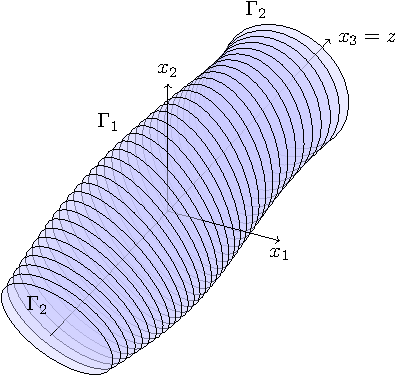
\includegraphics[width=0.25\textwidth]{figbound.pdf}}
  \end{tabular}
%%
$\Omega \subset \Re^3$. The $\Gamma_1$ forms the casing
of the pipe, while $\Gamma_2$ is the open boundary at the inlet and
outlet of the beam pipe, respectively.  
The Poisson problem with Robin boundary condition is given by:
\begin{equation*} \label{eq:poisson}
  \begin{gathered}
    -\epsilon_0\, \Delta \phi = \rho\ \text{in}\ \Omega, \\
    \phi = g \equiv 0\ \text{on}\ \Gamma_1, \quad
    \partial_n{\phi} +  (1/d) \phi = 0\
    \text{on}\ \Gamma_2.
  \end{gathered}
\end{equation*}
We discretize by a standard second order finite
difference scheme defined on a rectangular grid.
The boundary conditions are satisfied by constant, linear, or quadratic
extrapolation.

The finite difference discretization just described leads to a system of
equations
\begin{equation*} \label{eq:lin-syst}
  A \mathbf{x} = \mathbf{b}.
\end{equation*}
To improve the convergence behavior of the used CG methods we
precondition by smoothed aggregation-based algebraic
multigrid (SA-AMG) preconditioner.  
The multigrid preconditioner and iterative solver are implemented with
the help of the Trilinos framework.
\vspace{-0.4em}
  }

%%%%%%%%%%%%%%%%%%%%%%%%%%%%%%%%%%%%%%%%%%%%%%%%%%%%%%%%%%%%%%%%%%%%%%%%%%%%%%
  \headerbox{\sf PSI 590 MeV Ring Cyclotron}{name=se,column=0,span=1,above=bottom}{
%%%%%%%%%%%%%%%%%%%%%%%%%%%%%%%%%%%%%%%%%%%%%%%%%%%%%%%%%%%%%%%%%%%%%%%%%%%%%%
\sf The 1.3 MW of beam power delivered by the PSI 590 
MeV Ring Cyclotron together with stringent requirements 
regarding the controlled and uncontrolled beam losses 
poses great challenges with respect to predictive simulations \cite{BI}.
\begin{center}
 \begin{tabular}{cc}
       \hspace{-0.2em}\scalebox{1}{\includegraphics[width=0.99\textwidth]{Screen.pdf}}
 \end{tabular}
 \end{center}
 {\small The radial beam profiles with indicated turn numbers at extraction for a 2 mA beam. Excellent agreement
 between \opalcycl simulations and measurement is obtained. }
 \vspace{1.5em}
 }

%%%%%%%%%%%%%%%%%%%%%%%%%%%%%%%%%%%%%%%%%%%%%%%%%%%%%%%%%%%%%%%%%%%%%%%%%%%%%%%
%  \headerbox{\sf Future Work}{name=references,column=2,below=FN}{
%%%%%%%%%%%%%%%%%%%%%%%%%%%%%%%%%%%%%%%%%%%%%%%%%%%%%%%%%%%%%%%%%%%%%%%%%%%%%%%
% \sf
%      \begin{itemize}
%        \item 3D FEM Time Domain Maxwell Solver 
%        \item 3D CSR Time Domain Maxwell Solver
%        \item Multiobjective optimization (Pareto sense)
%        \item \opalmap 3D space charge and operator splitting
%        
%      \end{itemize}
% }





%%%%%%%%%%%%%%%%%%%%%%%%%%%%%%%%%%%%%%%%%%%%%%%%%%%%%%%%%%%%%%%%%%%%%%%%%%%%%%
  \headerbox{\sf References}{name=references,column=2,above=bottom}{
%%%%%%%%%%%%%%%%%%%%%%%%%%%%%%%%%%%%%%%%%%%%%%%%%%%%%%%%%%%%%%%%%%%%%%%%%%%%%%
  
    \smaller
    \vspace{-0.4em}
    \bibliographystyle{ieee}
    \renewcommand{\section}[2]{\vskip 0.05em}
      \begin{thebibliography}{1}\itemsep=-0.01em
      \setlength{\baselineskip}{0.4em}
    \bibitem{OP}\sf A. Adelmann et.al ,
      The OPAL (Object Oriented Parallel Accelerator Library) 
              Framework, Paul Scherrer Institut, PSI-PR-08-02, 2008-2010
\bibitem{SV}\sf A. Adelmann, P. Arbenz and Y. Ineichen, 
J. Comp. Phys, 229 (12): 4554-4566 (2010)
\bibitem{SCH}\sf T. Schietinger et.al, LINAC10, TUP009, (2010)     
\bibitem{BI}\sf Y.Bi et.al, HB2010, TUO2A03, (2010)     

      \end{thebibliography}
  \vspace{0.5em}     
 }

%%%%%%%%%%%%%%%%%%%%%%%%%%%%%%%%%%%%%%%%%%%%%%%%%%%%%%%%%%%%%%%%%%%%%%%%%%%%%%
  \headerbox{\sf Electron Linac Modeling}{name=bench,column=1,span=1,above=bottom}{
  \vspace{-1mm}
%%%%%%%%%%%%%%%%%%%%%%%%%%%%%%%%%%%%%%%%%%%%%%%%%%%%%%%%%%%%%%%%%%%%%%%%%%%%%%
\sf The Paul Scherrer Institut is commissioning a 250
MeV injector test facility in preparation for the SwissFEL
project \cite{SCH}. Its primary purpose is the demonstration of a highbrightness
electron beam meeting the specifications of the
SwissFEL main linac and undulator complex.
\begin{center}
 \begin{tabular}{cc}
       \hspace{-0.2em}\scalebox{1}{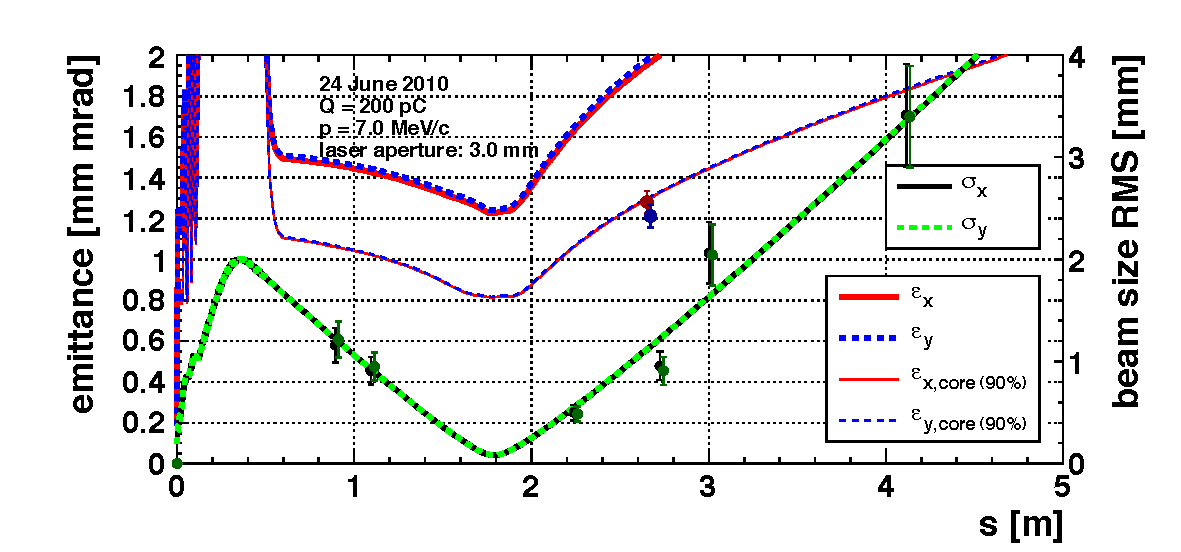
\includegraphics[width=1.\textwidth]{./250MeV-1.pdf}}
 \end{tabular}
 \end{center}
 {\small \sf Here we show an example, for the very first part of the injector (up to 6.7 MeV). Measurement of the beam envelope and normalized emittance for a charge of 200~pC,  together with a matched 3D \opalt simulation
 agreeing very well.
 We are about to extend this for the full 250 MeV injector test facility.}
 \vspace{0.5em}

}
%
\end{poster}%
\end{document}
